\documentclass[a4paper,12pt]{article} % добавить leqno в [] для нумерации слева
\usepackage[a4paper,top=1.3cm,bottom=2cm,left=1.5cm,right=1.5cm,marginparwidth=0.75cm]{geometry}

\usepackage[warn]{mathtext}
\usepackage[T2A]{fontenc}
\usepackage[utf8]{inputenc} 
\usepackage[english, russian]{babel}

\usepackage{ upgreek }
\usepackage[table,xcdraw]{xcolor}

\usepackage{indentfirst} %tabutation

\usepackage{amsmath, amsfonts, amssymb, amsthm, mathtools, mathtext} 

\usepackage{graphicx}

\usepackage{wrapfig}
\usepackage{tabularx}



%%% Дополнительная работа с математикой
\usepackage{amsmath,amsfonts,amssymb,amsthm,mathtools} % AMS



%% Шрифты
\usepackage{euscript}	 % Шрифт Евклид
\usepackage{mathrsfs} % Красивый матшрифт


%%% Заголовок
\author{Устюжанина Мария Алексеевна}
\title{Лабораторная работа №1.1.1

Измерение удельного сопротивления нихромовой проволоки
}
\date{\today}

\begin{document}

\begin{titlepage}
	\begin{center}
		{\large МОСКОВСКИЙ ФИЗИКО-ТЕХНИЧЕСКИЙ ИНСТИТУТ (НАЦИОНАЛЬНЫЙ ИССЛЕДОВАТЕЛЬСКИЙ УНИВЕРСИТЕТ)}
	\end{center}
	\begin{center}
		{\large Физтех-школа радиотехники и компьютерных технологий.}
	\end{center}
	
	
	\vspace{4.5cm}
	{\huge
		\begin{center}
			{\bf Отчёт о выполнении лабораторной работы 1.1.1}\\
			 Определение систематических  случайных погрешностей при измерении удельного сопротивления нихромовой проволоки.
		\end{center}
	}
	\vspace{2cm}
	\begin{flushright}
		{\LARGE Автор:\\ Устюжанина Мария Алексеевна \\
			\vspace{0.2cm}
			Б01-107}
	\end{flushright}
	\vspace{8cm}
	\begin{center}
		Долгопрудный 2021
	\end{center}
\end{titlepage}

\section{Введение}

\textbf{Цель работы:} измерить удельное проволоки, изготовленной из нихромового сплава, и вычислить систематическую и случайную погрешности при использовании измерительных приборов(штангенциркуля, микрометра, мультиметра, амперметра, моста постоянного тока).
\medskip
\textbf{Оборудование:} штангенциркуль, микрометр, отрезок проволоки из нихрома, амперметр, мультиметр, источник ЭДС, мост постоянного тока, реостат, ключ.
\medskip

\section{Теоретические сведения}
Методы измерения сопротивления:
\begin{enumerate}
	\item определение углового коэффициента наклона зависимости напряжения на проволоке от тока через неё;
	\item измерение с помощью моста постоянного тока.
\end{enumerate}

Удельное сопротивления однородной проволоки круглого сечения можно определить по следующей формуле:


\[\rho = R \frac{\pi d^2}{4l},\]


\noindent где $R$ -- сопротивление проволоки, $d$ -- её диаметр, $l$ -- длина.

\medskip

\begin{wrapfigure}[17]{r}{0.2\linewidth} 
\vspace{-5ex}
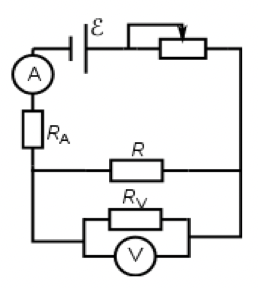
\includegraphics[width=\linewidth]{scheme1}
\caption{Схема цепи}
\label{fig:somelabel}
\end{wrapfigure}

Согласно закону Ома напряжение $V$ и ток $I$ в образце связаны соотношением


\[V = RI.\]

Для измерения напряжения и тока используем схему, изображенную на рис.1. Так как она приводит к меньшей поправке.
\medskip

Ввиду неидеальности используемого вольтметра необходимо учесть поправку на его конечное сопротивление $R_V$. Показания амперметра $I_A$ и вольтметра $V_B$ связаны соотношением:

\[V_B = R'I_A,\]

где R' — сопротивление параллельно соединённых проволоки и вольтметра.

\medskip

При этом $\frac{1}{R^\prime} = \frac{1}{R_V} + \frac{1}{R}$, и $R_V \gg R, R'$.\\

Таким образом, график зависимости $V_\text{В}\left(I_A\right)$ должен представлять прямую, угловой коэффициент которой есть $R'$, откуда сопротивление образца может быть найдено по следующей формуле:


\[R = \dfrac{R_V R^\prime}{R_V - R^\prime} \approx R^\prime \left( 1 + \frac{R^\prime}{R_V} \right).\]

\section{Оборудование и экспериментальные погрешности}

\textbf{Штангенциркуль:} $\Delta_\text{шт} = \pm 0,1$ мм \\
\textbf{Микрометр:} $\Delta_\text{мкм} = \pm 0,005$ мм \\
\textbf{Вольтметр(в качестве вольтметра использовался мультиметр):} $R_v=10$МОм

\noindent \textbf{Амперметр:}

\begin{tabular}{|l|l|}
	\hline
	Система&Электромагнитная \\
	\hline
	Класс точности &0,2 \\
	\hline
	Предел измерения&300 мА\\
	\hline
	Число делений& 150 ед. \\
	\hline
	Цена деления&2 мА \\
	\hline
	Абс. погрешность &0.5 мА \\
	\hline
	Внутреннее сопротивление& $R_A = 0,55 $Ом \\
	\hline
\end{tabular}\\

\medskip

%В диапазоне измерения $R$ от 1 до 10 Ом относительная поправка к сопротивлению согласно ф-ле составляет $\approx 10^{-4} \% $ (при $ R^\prime=10 \text{ Ом} $ и $ R_V = 5 \text{ кОм} $). Поэтому эта поправка пренебрежимо мала и не оказывает значительного влияния на последующие измерения. Поэтому далее будем считать, что

%%%end{equation}\\

\noindent\textbf{Мост постоянного тока P4833:}\\
\begin{tabular}{|p{8cm}|p{7cm}|}
	\hline
	Класс точности&0,1 \\
	\hline
	Разрядность магазина сопротивлений& 5 ед. \\
	\hline
	Исследуемый диапазон измерений& $ 10^{-4} - 10 \text{ Ом} $ (для множителя $ N = 10^{-2} $) \\
	\hline
	Погрешность измерений в используемом диапазоне& $\pm0,010\text{ Ом}$ \\
	\hline
\end{tabular}\\

\section{Результаты измерений и обработка данных}

\subsection{Измерение диаметра $d$ проволоки}

Измерения проводились штангенциркулем и микрометром для $N = 10$ различных участков проволоки. При измерении штангенциркулем получено $d = 0,4$ мм для всех участков. При измерении микрометром были получены следующие показания:

\begin{table}[h]
	\begin{tabular}{|l|l|l|l|l|l|l|l|l|l|l|}
		\hline
		Номер   измерения & 1    & 2    & 3    & 4    & 5    & 6    & 7    & 8    & 9    & 10   \\ \hline
		d, мм             & 0,37 & 0,365 & 0,37 & 0,365 & 0,365 & 0,36 & 0,36 & 0,37 & 0,365 & 0,37 \\ \hline
	\end{tabular}\caption{\textit{Измерение диаметра проволоки микрометром}}
\end{table}

Среднее значение диаметра $ \overline{d} = \frac{\sum d_i}{N} = 0,366 \text{ мм}$.\\

Случайная погрешность измерения $ \sigma_{\overline{d}} = \sqrt{\frac{1}{N  (N-1)}\sum(d_i-\overline{d})^2} \approx 0,0012 \text{ мм}$.\\

С учётом инструментальной погрешности $ \Delta_\text{мкм} = 0,005$ мм погрешность диаметра может быть вычислена как $ \sigma^{\text{полн}}_{\overline{d}} = \sqrt{\sigma^2_{\overline{d}} + \Delta^2_{\text{мкм}}} \approx 0,005 \text{ мм}$. \\

\textit{Окончательные результаты измерения диаметра проволоки:}

\begin{itemize}
	\item Штангенциркулем: $ d = 0,4 \pm 0,1 \text{ мм}  $
	\item Микрометром:  $ \underline{(0,366 \pm 0,005 \text{ мм}})  $
\end{itemize}
\newpage
\subsection{Измерение сопротивления проволоки}
Проведем 10 измерений значений тока и напряжения для 3 длин проволоки. Результаты занесем в таблицу:



\begin{table}[h]
\noindent\begin{tabular}{|p{1,6cm}|p{1cm}|p{1cm}|p{1cm}|p{1cm}|p{1cm}|p{1cm}|p{1cm}|p{1cm}|p{1cm}|p{1cm}|}
		\hline
		\multicolumn{11}{|c|}{$ l = 20 $ см}                                                                    \\ \hline
		$ I_A $, дел. 
		&32,5&38& 42,5& 49& 55& 66,5& 78& 91& 103,5& 135\\ \hline
		$ I_A$, мA &
		35&
		76& 85& 98& 110& 133& 156& 182 & 207 & 27
\\ \hline
		$ V_B $, В      & 0,1321 & 0,1563 & 0,175 & 0,2017 & 0,2248 & 0,2735 & 0,3217 & 0,3746 & 0,51  \\ \hline


		\multicolumn{11}{|c|}{$ l = 30 $ см}                                                                    \\ \hline
		$ I_A $, дел. & 34    & 37,5  & 42,5  & 48   & 52,5  & 58,5  & 70    & 77,5  & 91,5  & 118    \\
 \hline
		$ I_A$, мA    &  68    & 75    & 85    & 96   & 105   & 117   & 140   & 155   & 183   & 236    \\
 \hline
		$  V_B $, В  & 0,219 & 0,241 & 0,274 & 0,31 & 0,339 & 0,381 & 0,455 & 0,504 & 0,596 & 0,7685 \\
 \hline


		\multicolumn{11}{|c|}{$ l = 50 $ см}                                                                    \\ \hline
		$ I_A $, дел. & 32&	38&	47&	54,5&	64	&71,5	&82&	86&	98&	118,5    \\ \hline
		$ I_A$, мA      & 64&	76&	94&	109&	128&	143&	164&	172&	196&	237    \\ \hline
		$  V_B $, В     & 0,341&	0,411&	0,503&	0,589&	0,691&	0,771&	0,885&	0,929&	1,067&	1,288 \\ \hline
	\end{tabular}
\end{table}

 Графики зависимостей $U=f(I)$ для всех отрезков проволоки:
\begin{figure}[h]
\centering
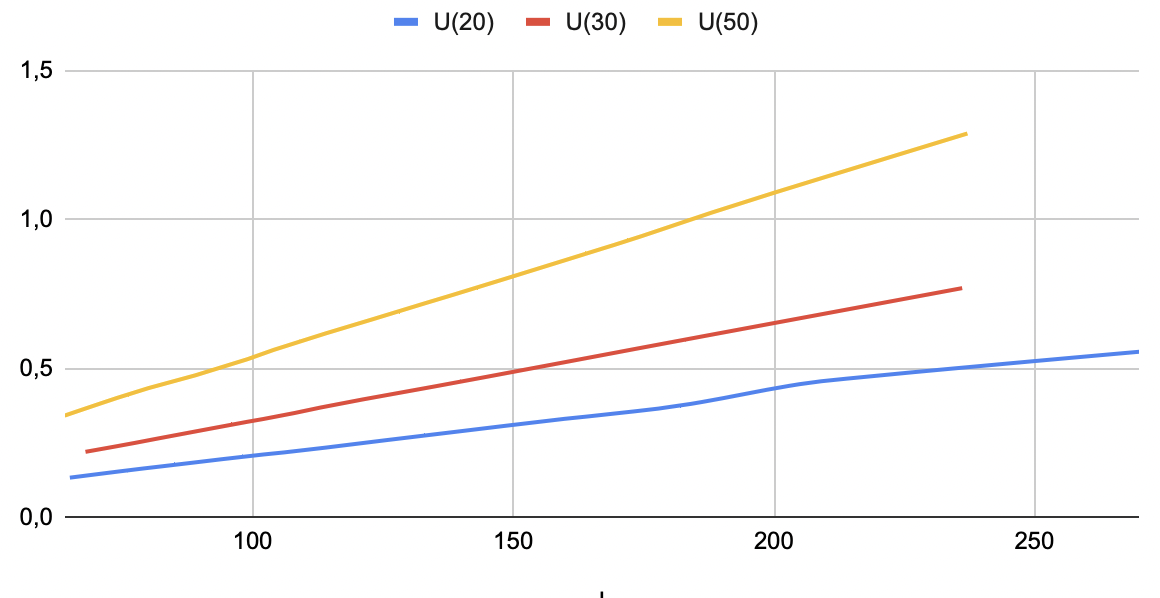
\includegraphics[width=0.6\linewidth]{Гр1}
\label{fig:mpr}
\end{figure}

Из графиков видно, что нет различия между значениями, полученными при возрастании и при уменьшении тока.

Для каждой длины проволоки находим сопротивление $R_{ср}=\frac{<UI>}{<I^2>}$ и среднеквадратичную случайную ошибку:
\[\sigma^{случ}_{R_{ср}} = \frac{1}{\sqrt{10}}\sqrt{\frac{<U^2>}{<I^2>}-R^2_{ср}},\]

где 10 - число экспериментальных точек.

Возможную систематическую погрешность $R_ср$ найдем по формуле:

\[\sigma^{сист}_{R_{cр}} = R_{ср}\sqrt{(\frac{\sigma U}{U})^2+(\frac{\sigma I}{I})^2,}\]

где U, I - максимальные значения силы тока и напряжения, $\sigma U, \sigma I$ - ошибки измерения вольтметром и амперметром:

\[\sigma U = 0,1 мВ\]

\[\sigma I = 1 мА\]

 Ошибка измерений $\sigma_R = \sqrt{(\sigma^{случ}_R)^2 +  (\sigma^{сист}_R)^2}$

Результаты в таблице.

\subsection{Измерения сопротивления с помощью мультиметра и моста}

Измерим сопротивление с помощью мультиметра $R_0$ и моста "постоянного тока"  $ R_0'$. Занесем результаты в таблицу.

Для всех длин вычислим поправку в измеренное значение по формуле: 

\[ R_{пр} = R_{ср} + \frac{R_{ср}^2}{R_V} \]


Занесем разультаты в таблицу.

\medskip

\textbf{Результаты измерения сопротивления проволоки и погрешность}
\

\

    \begin{tabular}{|l|l|l|l|}
    \hline
    l, см      & 20     & 30     & 50     \\ \hline
    Rcр        & 2,079  & 3,249  & 5,412  \\
    $R_0$       & 2,03   & 3,22   & 5,4    \\
    $R_0'$      & 2,2156 & 3,3977 & 5,4974 \\ \hline
    $\sigma_{сист}$ & 0,008  & 0,014  & 0,023  \\
    $\sigma_{случ}$ & 0,015  & 0,004  & 0,008  \\
    $\sigma_{полн}$ & 0,017  & 0,015  & 0,26   \\ \hline
    \end{tabular}
\

\

\textbf{Итоговый результаты измерения сопротиивления проволоки и погрешность}
\

\

    \begin{tabular}{|l|l|l|l|}
    \hline
    l, см       & 20    & 30    & 50    \\ \hline
    Rcр         & 2,079 & 3,249 & 5,412 \\ \hline
    $\sigma_{полн}$ & 0,017 & 0,015 & 0,024 \\ \hline
    \end{tabular}

\

\

Сравнивая результаты измерения сопротивления проволоки с помощью вольтметра и амперметра с результатами, полученными с помощью моста и мультиметра получаем расхождения в значениях, не превышающие погрешности.

\subsection{Нахождение удельного сопротивления проволоки}

\[ \rho = \frac{R_{пр}\cdot \pi d^2}{4l}\]

И погрешность по формуле:

\[\frac{\sigma_{\rho}}{\rho}=\sqrt{(\frac{\sigma R}{R})^2+(2\frac{\sigma d}{d})^2+(\frac{\sigma l}{l})^2}\]

\

\

    \begin{tabular}{|l|l|l|}
    \hline
    l, см & $\rho, 10^{-6} Ом\cdotм $ & $\sigma_\rho, 10^{-6} Ом \cdot м$ \\ \hline
    20    & 1,09        & 0,17         \\
    30    & 1,14        & 0,16         \\
    50    & 1,14        & 0,16         \\ \hline
    \end{tabular}


\

\

Тогда: \[ \rho = (1,12\pm 0,17) \cdot 10^{-6} Ом \cdot м\]
\newpage

\section{Вывод}
Сравним табличное значение с полученным: табличные лежат удельного сопротивления нихромовой проволоки лежат в диапазоне $0,97...1.14 \cdot 10^{-6} Ом\cdot м$. Полученные значения попадают в этот диапазон.

Использованный в работе метод позволил получить результат с точностью 14,7\%. 

В ходе работы был подтвержден закон Ома для участка цепи. Установленно, что сопротивление проволоки не зависит от величины I и U, а зависит только от их отношения.

В ходе эксперемента было выявлено, что с увеличением длины проволоки систематическая погрешность увеличивается. В полную погрешность вносят существенный вклад и систематическая, и случайная погрешности.

\end{document}